\documentclass[landscape, 10pt]{article}
\usepackage[margin=2cm]{geometry}
\usepackage{multicol,microtype,color,amsmath,amsthm,amssymb, dsfont,mathdots, alltt, parskip, pgf, tikz}
\usetikzlibrary{arrows,automata}
%\usepackage[T1]{fontenc}
%\usepackage[latin9]{inputenc}
\newcommand{\N}{\mathbb{N}}
\newcommand{\Z}{\mathbb{Z}}
\newcommand{\C}{\mathbb{C}}
\newcommand{\R}{\mathbb{R}}
\newcommand{\ep}{\epsilon}
\newcommand{\epm}{\epsilon_{machine}}
\newcommand{\norm}[1]{\parallel \!#1 \!\parallel}
\newcommand{\po}[2]{\textbf{#1} #2}
\def\ci{\perp\!\!\!\perp} % from Wikipedia
\def\d{\delta}
\begin{document}
\title{Sum-Product notes}
\maketitle

$$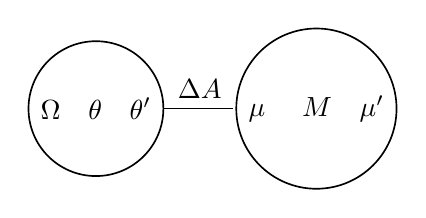
\begin{tikzpicture}[-,>=stealth',shorten >=1pt,auto,node distance=2.8cm,
                    semithick]
  \tikzstyle{every state}=[fill=none,draw=black,text=black]
\node[state]         (A) {$\Omega\ \ \ \theta\ \ \ \theta'$};
  \node[state] (B)     [right of=A] {$\mu\ \ \ \ M\ \ \ \mu'$};

  \path (A) edge              node {$\Delta A$} (B);
\end{tikzpicture}
$$

$\mu=\Delta A \Theta$
Given any point $\mu$ there exists a $\theta$.  Given any point $\mu ' $ there is a $\theta '$.\\
When is the map 1-1?  When the exponential family is not minimal.  Variational methods are about moving from one representation to another.\\
When it is 1-1, $(\Delta A)^{-1}$ exists.\\
$A\theta=\sup_{\mu\in M}\{\left<\theta,\mu\right>-A^*(\mu)\}$\\
This is discrete over complete sufficient statistics.\\
$P_\theta(x)=\exp\{\sum_s\theta_s x_s + \sum_(s,t\in E)(x_s x_t)$\\
$\theta_s=\sum_{j,i}\theta_{s_{ij}}\perp_{sj}(x,s)$\\
\subsection*{Pseudo-marginals}
$$
\mu=
\begin{cases}{ll}
\mu_s(x_s) & $Nodewise$\\ 
\mu_{st}&(x_s,x_t-$Pairwise marginals of some distribution $P\\
\end{cases}
$$
$\mu_{st}$ is only defined over edges of $G$.\\

$$\mathds{L}_G=
\begin{cases}{ll}
T_s(x_s)&s\in V
\\T_{st}&(s,t)\in E\end{cases}$$
Norm $\sum_{x_s}T_sx_s=1$\\
Marginals $\sum_{x_{s}} T_{st}(x_sx_t)=T_t(x_t)$\\
Marginals $\sum_{x_{t}} T_{st}(x_sx_t)=T_t(x_t)$\\
Prop$(I) \mathds{L}G \supseteq M(G)$\\
If $\mu\in M(G)$ it satisfies norm and marginal constraints $\rightarrow \mu \in \mathds{L}G$\\
There are exponential constraints for $\mu$ and linear ones for $\mathds{L}(G)$\\
$$
\begin{array}{ll}
P(x_1,\dots, x_n)
\mu_i(x_i)&=P(x_i)\\
\mu_{i,j}(x_ix_j)&=P(x_i,x_j)
\end{array}
$$
If graph $G$ is a tree $T$, then $\mathds{L}(T)=\mu(T)$ because nodewise and pairwise marginals are all we need.

\textit{Proof}\\
$L(G)\supseteq\mu_G$ (Shown).  We want to show that $\mathds{L}(T)\subseteq\mu_T$.  We will take a $\mu\in\mathds{L}(T)$ such that it satisfies marginal constaints and show that it is consistent with regard to a joint distribution.

$\mu_s(x_s),s\in V$\\
$\mu_{st}(x_s)(x_t),(s,t)\in T$\\
$P_{\mu}(x)=\Pi_{s\in V} \mu_s(x_s)\Pi_{s,t \in E} \frac{\mu_{st}(x_sx_t)}{\mu_s(x_s)\mu_t(x_t)}$ such that $\mu$ is consistent with regard to $P_\mu$.

We can compute the Bethe-entropy of the tree-structure distribution.  Suppose we have a tree-structured distribution with mean parameters $\mu$.  Then we can write down the distribution in terms of $\mu.$\\
$$
\begin{array}{ll}
A^*_(\mu)&=$entropy$(P_\mu)\\
	&=\mathds{E}_{pm}|\log P_\mu(x)|\\
	&=\mathds{E}_{pm}|\sum_{s\in V}\log\mu_s(x_s)+\sum_{s,t\in E}\log\frac{\mu_{st}(x_s,x_t)}{\mu_s \mu_t}|\\
	&=-\sum_s\mathds{H}_s<\mu_sright>-\sum_{s,t\in E}I_{s,t}(\mu_{s,t})\\
\mathds{H}_{Bethe}(\mu)&=\sum_{s\in V}\mathds{H}_s(\mu_s)-\sum_{s,t\in E}I_{s,t}(\mu+{s,t})\\
	&= -A^*(\mu) $Exactly when $G$ is a tree$\\
\end{array}
$$

Computing entropy in the general case is NP-hard, but we can approximate it when $G$ is not a tree using the variaitonal principle.

We can aproximate to $A(\theta)$ as so:
$A_{Bethe}(\theta)=\sup_{\mu\in\mathds{L}(G)}\{ <\theta, \mu>+\mathds{H}_{Bethe}(\mu)-I\}$

We get sum-product from the fixed point update driven solution of optimization problem I.

$\mu_{st}(x_t)=\Psi_{st}(x_s,x_t)\Pi_{v\in N(S)_t}\mu_{v_s)}(x_s)$\\
This is a nonconvex problem.  If we do coordinate descent on the dual, we can get to a \textit{local} minimum. Regular sum-product often oscillates between very large ($O(v^2)$) parameters.

\subsubsection*{Reparamaterization}
Suppose we solve sum-product to a local minimum $\tau^*$ (a local minimum of $J$). Then $P_{\tau^*}(x)=I\Pi_{s\in V}T^*_s(x_s)\Pi_{s,t\in E} \frac {T^*_{st}(x_s,x_t)}{T^*_s(x_s)T^*_t(x_t)}$\\

We know that if $G$ is a tree and $T^*=\mu^*$, then $P_{T^*}=P_\theta$ and $P_{T^*}(x)=P_\theta(x)$\\

So it always holds that $P_\theta(x)=P_{T^*}(x)$\\

\subsection*{Hypergraphs}

Define a hypergraph $G\in(V,E)$ with nodes $v\in V$ and hyperedges $e\in E$ such that $e\subseteq E$.  A normal graph is a hypergraph with 2-node edges.

We can write the following graph as $E=(1,2)(2,3)(1,4)(2,4)$ or we can write $E=(1,2,4),(2,3)$
$$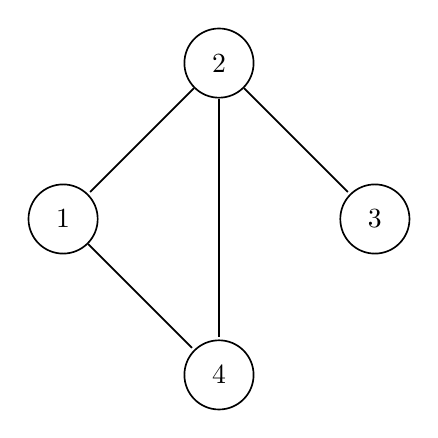
\begin{tikzpicture}[-,>=stealth',shorten >=1pt,auto,node distance=2.8cm,
                    semithick]
  \tikzstyle{every state}=[fill=none,draw=black,text=black]
\node[state]         (B) {$2$};
  \node[state] (A)     [below left of=B] {$1$};
  \node[state]         (C) [below right of=B] {$3$};
  \node[state]         (D) [below left of=C] {$4$};

  \path (B) edge              node {} (A)
        (B) edge        node {} (C)
        (B) edge        node {} (D)
        (A) edge        node {} (D);
\end{tikzpicture}
$$

Suppose we have the hypergraph with edges $E=(1,2,4),(2,3),(1,2),(2)$.  Then we have a \'node\' for each superedge and we connect $h\rightarrow g$ if $g\in h$. These form a partially ordered set with regard to set inclusion.

$$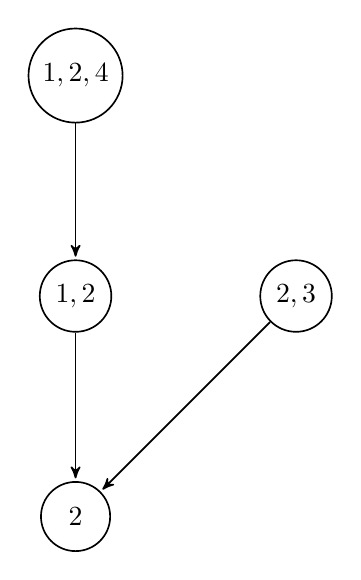
\begin{tikzpicture}[->,>=stealth',shorten >=1pt,auto,node distance=2.8cm,
                    semithick]
  \tikzstyle{every state}=[fill=none,draw=black,text=black]
\node[state]         (A) {$1,2,4$};
  \node[state] (B)     [below of=A] {$1,2$};
  \node[state]         (C) [below of=B] {$2$};
  \node[state]         (D) [right of=B] {$2,3$};

  \path (A) edge              node {} (B)
        (B) edge        node {} (C)
        (D) edge        node {} (C);
\end{tikzpicture}
$$

A general graphical model has subsets over cliques.  The hypergraph edges correspond to cliques.  We can do inference on these cliques.

Given a set of sufficient statistics $\mathds{L}(G)=T_n(x_n)$, such that $\sum_nT_n(x_n)=1$ we have $g,h$ such that $f\subseteq h$:

$\sum_{x_h} |x_gT_n(x_n)=T_g(x_g)|$

For the following graph

$$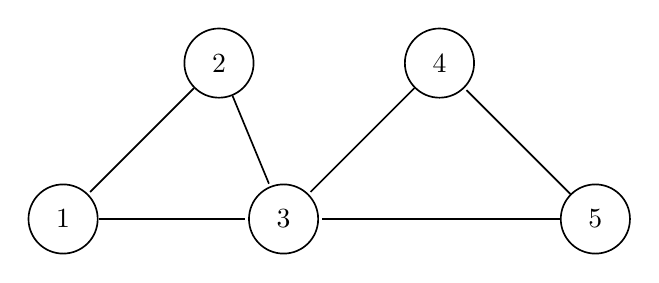
\begin{tikzpicture}[-,>=stealth',shorten >=1pt,auto,node distance=2.8cm,
                    semithick]
  \tikzstyle{every state}=[fill=none,draw=black,text=black]
\node[state]         (A) {$2$};
  \node[state] (B)     [right of=A] {$4$};
  \node[state]         (C) [below left of=A] {$1$};
  \node[state]         (D) [below right of=B] {$5$};
  \node[state]         (E) [below left of=B] {$3$};

  \path (A) edge              node {} (E)
        (A) edge        node {} (C)
        (B) edge        node {} (E)
        (D) edge        node {} (E)
        (C) edge        node {} (E)
        (D) edge        node {} (B);
\end{tikzpicture}
$$

(1, 2, 3) and (3, 4, 5) must be consistent.


$H_{hypertree}(\mu)=\sum_{n\in E}c(h)H_h(\mu_k)$ where $c(h)$ are overcounting numbers.\\
$\sup_{\mu\in\mathds{L}_G}\{<\theta,\mu>+H_{HT}(\mu)\}$




Message passing here is generalized beleif propagation.

\end{document}